This chapter will cover types of tests that ware used in this project.
It is a good practise to write special code that can check whether parts of the application work as intended.
This code is simply called tests.
This is not only useful to test the application parts when they are being written, but these tests could be run in future to ensure that possible code changes did not break the functionality of previously written parts.

% We will be using libraries Hamcrest and MockK.
% Hamcrest will be used for matching lists and MockK for mocking.

\section{Local unit tests}
These are tests that require only JVM.
They do not need any part of the Android framework, so there is no need to run them on an Android device, which makes them fast.
Parsing objects from JSON and back can and will be tested here.

\begin{figure}\centering
	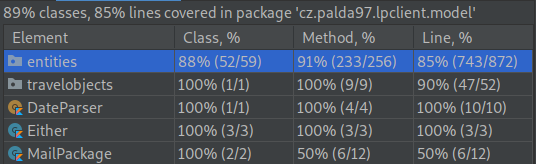
\includegraphics[width=1\textwidth]{pics/coverage.png}
	\caption[Test Coverage]{Picture with local test coverage}\label{fig:coverage}
\end{figure}

The model layer will be tested here, but since database is not accessible here, repository and DAOs will be excluded from these tests, alongside with some generated code, like from the Retrofit library.
The coverage, as displayed in \autoref{fig:coverage}, is 89 \% for classes and 85 \% for methods.
Coverage of 70 \% to 80 \% is commonly considered good coverage.

\section{Instrumented unit tests}
Instrumented tests require some part of the Android framework, so they run in background on an Android device.
Previously mentioned library Room (in \autoref{subsec:daoandnetwork}) requires a part of Android framework, so it can be used here.
Repositories will be tested here too.

Unfortunately, the coverage could not be put into operation here.
After researching how coverage can be done on instrumented tests, most of the tutorials are bound to various forks of JaCoCo library \cite{jacoco}, which caused some errors during commissioning attempts.
